\chapter{Background}
\label{sec:background}
This chapter presents the background information of the
thesis. Section~\ref{sec:mobile-robotics} gives an introduction into the
thesis' contxt of moble robotics and reasoning. In
Section~\ref{sec:robocup} we introduce the primary application and
evaluation domains, the RoboCup Logistics League (RCLL) and the
RoboCup@Home league. Afterwards, we present the software context with
robot software frameworks in
Section~\ref{sec:robot-software-frameworks}, planners and reasoners in
Section~\ref{sec:planners}, and databases in
Section~\ref{sec:databases}.

\section{Mobile Robotics and Reasoning}
\label{sec:mobile-robotics}
A robot is \emph{a machine capable of automatically carrying out a
  complex series of movements}~\cite{robot-dict} and belongs to the
group of \emph{cyber physical systems (CPS)}, which can be defined
as \emph{computing elements combined with physical sensing and
  interaction}~\cite{chapter-cps}. In contrast to mounted assembly
line robots, we focus in this thesis on autonomous mobile robots, thus
robots that are \emph{capable of moving in their environment} and
are \emph{capable of operating without any form of external control
  for extended periods of time}~\cite{autonomous-robots}. These robots
interact with their environment to fulfill a specific task they are
designed for. They are \emph{agents}, which utilize a
\emph{sense-think-act cycle}. Sensors are used to percieve the
environment, a computation device to decide what to do, and actuators
to interact with the environment. How a autonomous mobile robots can
acts depending on its sensing depends on its \emph{agent
  architecture}. Russell and Norvig differentiate the class of simple
\emph{reflex agents} and the class of more advanced
\emph{model-based, goal-based, and learning
  agents}~\cite{aimodern}. Reflex agents can only use the current
perception to compute how to react and are thus limited in their
capabilities because they can not remember anything from previous
cycles. All other agent architectures have an internal state, which
allows to take the perception history into account and implement more
complex behavior.

\subsection{Robot Memories}
\label{sec:robot-memories}
We define a \emph{robot memory} as a system that memorizes the
internal state of a robot between two or more sense-think-act
cycles. In the case of a model-based agent, it can include a model of
the robots environment to compensate for partial observability of the
domain. A goal-based agent remembers the given goal to achieve in the
environment and a learning agent remembers what was learned from
previous observations~\cite{aimodern}.

Physically, a robot memory can be stored on \emph{volatile} or
\emph{non-volatile} devices that can be read and written. A volatile
device, such as \emph{Random-access memory (RAM)}, can only store
information as long as it is powered. Usually, RAM acts as storage
when the internal state of the robot is represented by variables in
the programming language(s) used to implement the behavior of the
robot.  A non-volatile device, such as a hard disk drive, also keps
the information when it is not powered. Also a combination of volatile
and non-volatile devices can be used for storage as in this thesis. A
robot memory that is stored on a non-volatile device is called
\emph{persistent}.

\subsection{Knowledge Sharing}
\label{sec:knowledge-sharing}
A robot memory is not necessarily limited to a single robot. In a
\emph{multiagent system}, a system that is composed of multiple
interacting agents~\cite{multiagentsystems}, the agents can share
their internal state. In this case, the robot memory is called
\emph{distributed}. Furthermore, we will also call a system composed
of multiple interacting autonomous mobile robots a \emph{multi-robot
  system}. Similarly, a robot memory can also be shared on a single
robot between multiple agent programs that each implement a part of
the robots behavior. The architecture of a multiagent system can be
\emph{centralized} or \emph{distributed}. In the centralized one,
a central unit stores all relevant information and/or decides which
actions each agent should execute. In the distributed one, the
relevant information is stored and synchronized on all agents and/or
each agents makes it's own decisions. This also introduces the need of
\emph{consistency}, which requires that information stored in a
distributed system does not represents contradicting assumptions.
\todo[inline]{Mention Master-Slave vs. Peer-to-peer?}
\todo[inline]{Give Example (RoboEarth)?}

\subsection{Reasoning}
\label{sec:reasoning}
\todo[inline]{Write}

\section{RoboCup}
\label{sec:robocup}
\todo[inline]{check parallelity}
\emph{RoboCup} is an international robotics competition founded to
foster research in the field of robotics and artificial
intelligence~\cite{RoboCup-Paper}. It provides standardized problems
as a platform to compare research results. Teams from all over the
world compete in different leagues to benchmark their algorithms and
robotic systems. An special challenge of the RoboCup is making the
robotic system robust against real world complexity and challenges,
such as changing light conditions and unknown obstacles.

RoboCup features a variety of leagues, from soccer leagues in
different sizes to rescue robots, each focusing on another aspect or
application domain of robotics and artificial intelligence.  For
example there are soccer simulation leagues and small soccer robots
focusing on tactical team moves, humanoid soccer robots focusing on
body control and limited perception, and rescue robots, both fully
autonomous and partially tele-operated.  \todo[inline]{references rc
  leagues} The majority of the RoboCup leagues host soccer robots in
different sizes and complexities. The leagues range from the
\emph{Small Size League} with small cylindrical robots and ground
truth perception from an overhead camera to humanoid robots in teen
size which need to have all sensors and computation devices on the
robot. The RoboCup also features more application oriented domains,
e.g. the \emph{Rescue League} with robots solving different challenges
in desaster scenarios and \emph{RoboCup@Work} with robots operating in
an industrial scenario to perform identification, handling and
transporting tasks with work related objects, such as skrews and
nuts. In the following, we describe the \emph{RoboCup Logistics League
  (RCLL)}, which features logistics robots in a production scenario,
and the \emph{RoboCup@Home} leage featuring service robots in a
domestic environment in more detail. These two leagues are used as
application and evaluation domains of the thesis.

\subsection{RoboCup Logistics League}

The \emph{RoboCup Logistics League (RCLL)}\footnote{RoboCup Logistics
  League website: \url{http://www.robocup-logistics.org}} is an
industry-oriented competition~\cite{LLSF-Rules-2016}.
\todo[inline]{cite rcll mps paper} It tackles the problem of
production logistics in a smart factory, where mobile robots have to
plan, execute, and optimize the material and production flow between
machines to produce and deliver products according to dynamic
orders. Each competing team deploys a group of three robots that has
to build ordered products autonomously by interacting with
\emph{Modular Production Machines (MPS)} and transporting work pieces
between these machines.
\begin{wrapfigure}{r}{0.3\textwidth}
  \centering
  \vspace{-2.7ex}
  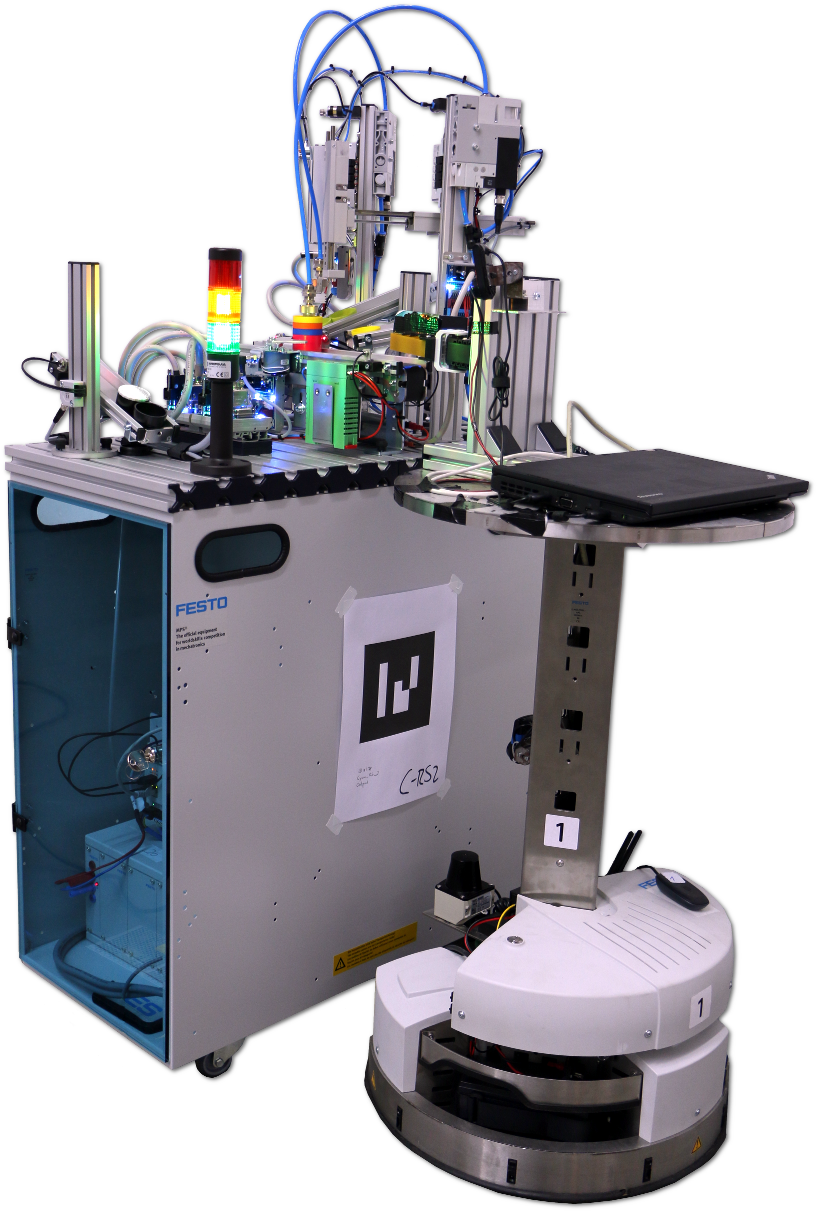
\includegraphics[width=0.3\textwidth]{img/rcll}
  \vspace{-4ex}
  \caption{Robot and MPS used in the RCLL~\cite{chapter-cps}}
  \label{fig:rcll}
\end{wrapfigure}
\reffig{fig:rcll} shows an RCLL robot filling a machine that mounts
colored rings on work pieces. The robots are based on the Festo
Robotino 3 platform, which uses a holonomic drive, and can be extended
and programmed by the teams. The robot shown in \reffig{fig:rcll} was
built by the Carologistics team and uses a laser range finder for
localization, a custom made gripper for handling work pieces, and
several cameras for detection of markers and light-signals mounted on
the machines~\cite{Carologistics2015,chapter-cps}. The game is
controlled by a software component called \emph{referee box (refbox)}
which randomizes the machine placement in the factory and the
production orders, communicates with participating robots, controls
machines, and awards points.

The game consists of two phases. In the first phase, the
\emph{exploration phase}, the robots have to roam the factory to find
randomly placed machines, which are used later. By detecting the
light signal shown by the machines, the robots can determine the
machine-type. For correct reports of discovered machines to the refbox
the team is awarded points, for incorrect ones points are subtracted.

\begin{figure}[t]
  \centering
  \begin{minipage}{.8\linewidth}
  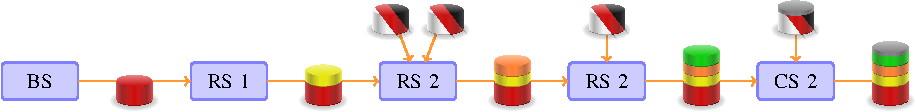
\includegraphics[width=\linewidth]{img/chain_c3}%
  \end{minipage}
  \quad%
  \begin{minipage}{.15\linewidth}
  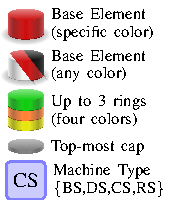
\includegraphics[width=\linewidth]{img/legend}%
  \end{minipage}
  \caption{Production chain of a high complexity
    product in the RCLL.}
  \vspace{-2mm}
  \label{fig:prod-chain}
\end{figure}

In the second phase, the \emph{production phase}, the refbox announces
orders, which products have to be produced by the robots. The products
are build from colored cups with optionally mounted rings and a
colored cap.  \reffig{fig:prod-chain} shows the production chain for
building a high complexity product.  There are four different machine
types. The \emph{base-station (BS)} provides new bases, the colored
cups, as raw resource. The \emph{ring stations (RS)} mounts colored
rings on a work piece after preparing it with a varying amount of
bases.  The \emph{cap-station (CS)} mounts black or grey caps to
finish a product after loading it with a cap form a shelf first.
Finally, the \emph{delivery-station (DS)} is used to deliver products.

A major challenge of the RCLL lies in the fully autonomous task
planning and coordination of the multi-robot system in the dynamic
environment with spatial information and time constraints. The
dynamism of the environment is caused by the ranomization of factory
layout, machine out-of-order times and ordered product composition and
unknown obstacles, such as the other teams robots. Furthermore,
baseline robotic challenges such as collision avoidance, perception
and behavior execution need to be solved. To outperform opponent
teams, the robots have to build as many ordered products as possible
and deliver them in time given time window.  To cope with these
challenges, a multi-robot decision making is necessary and therefore a
mechanism to share knowledge about the world model between the
robots. This can be done by the robot memory, which also allows
combining a global planner for finding plans and a reasoner for plan
execution.

\subsection{RoboCup@Home League}
The RoboCup@Home league is a competition about domestic service
robots~\cite{wisspeintner2009robocup}. Robots have to assist
humans in a wide variety of everyday tasks. These tasks include
serving
\begin{wrapfigure}{r}{0.3\textwidth}
  \centering
  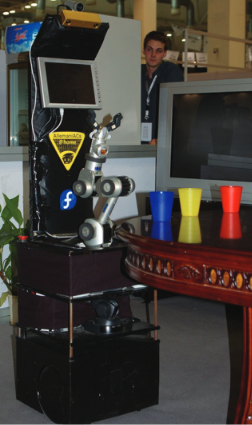
\includegraphics[height=150px]{img/ceasar}%
  \caption{RoboCup@Home robot tidying up~\cite{wisspeintner2009robocup}}
  \vspace{-3mm}
  \label{fig:athome}
\end{wrapfigure}
drinks, cleaning, setting tables, guiding or following people,
helping in emergency situations, shopping, and cooking.
\reffig{fig:athome} shows an @Home robot in the
competition.
%
The goal of the RoboCup@Home league is to foster and benchmark
research in the area of domestic service robots, to build a research
community and to envision autonomous multi-purpose robots helping
humans and especially elder people in the personal life.

The competition consists of multiple sub-tasks,
such as finding and manipulating objects, navigation tasks,
remembering persons, wait on tables, acting as
nurse, and an open challenge~\cite{athome-rules}.
To solve these challenges, robots need to
have a wide variety of abilities, including navigation, object
detection and manipulation, speech recognition, and especially human
robot interaction, which requires, for example, applying everyday
knowledge to incomplete task descriptions given by humans.

Important challenges in the @Home league are acting robustly in a
dynamic and only partial observable domestic environment and hybrid
reasoning with symbolic and spatio-temporal information.
The robot memory can help here because it allows to collect a lot
of knowledge about the concrete domestic environment and, for example,
log object observations to learn their distribution~\cite{deebul}.
\todo[inline]{check deebul ref}
Furthermore, it can help with hybrid reasoning by transforming
spatio-temporal knowledge into symbolic knowledge with computables.
Furthermore, detecting and manipulating objects in a personal
environment can be difficult because the space the robot acts in, for
example the frige, can be very clouded.
\todo[inline]{introduce ceasar?}

\section{Robot Software Frameworks}
\label{sec:robot-software-frameworks}
A \emph{robot software framework} can be defined as design and
implementation of a middleware for the implementation of a robot
control software~\cite{tnthesis}. \todo[inline]{add orcos ref 'desing
  and implementation'} It provides basic functionality,
infrastructure, and tools to develop robot software. Furthermore, it
can define a standard for component interfaces that allows building on
a variety of Open Source solutions for robotic problems. In the
following, we introduce the widely used Robot Operating System and
Fawkes, which is used in this thesis.
\subsection{Robot Operating System}
\label{sec:ros}
\todo[inline]{write}
\subsection{Fawkes}
\label{sec:fawkes}
\todo[inline]{review}
The basis for the proposed thesis is the robot software framework
\emph{Fawkes}\footnote{\url{http://www.fawkesrobotics.org}}, which is
available as open source~\cite{FawkesDesign,Fawkes-RCLL-2014}.
%and developed at the Knowledge-based Systems
%Group\footnote{\url{http://www.kbsg.rwth-aachen.de}} (KBSG) at RWTH
%Aachen University
It is designed to work with
various robots in different domains and follows a component-based
software design, which separates functional entities into individual
software modules~\cite{component}. This enables reusing
software solutions for robotic problems, such as localization,
perception, reasoning, and behavior execution. Compiled
components can be loaded as \emph{plugins} at run-time.
%
Plugin activity is organized in threads
%to make use of multi-core architectures. The threads
that can be run continuously ore hooked into
the main-loop of Fawkes to order the execution into a
\emph{sense-think-act} cycle.
%This guarantees that higher-level components can use the latest data.
Fawkes softly guarantees loop times by
monitoring and eventually pausing and resuming threads running for too
long.
% Ros blabla from BA?
Features in Fawkes are provided as \emph{aspects}. These are
based on aspect-oriented programming~\cite{aspect_oriented} and give
access to particular features. Threads that need to use a feature can
inherit from the corresponding aspect. For example, there are aspects
for accessing logging, timing, and specific external libraries~\cite{tnthesis}.

The communication between plugins is realized with a \emph{hybrid blackboard}
paradigm. The blackboard lists structured entries called
\emph{interfaces}, which contain qualitative and quantitative information.
Interfaces can be
provided by one plugin at a time, the writer, and read by other
plugins, the readers. This allows a flexible communication
because the interface is independent from the concrete writer and readers.
For example, sensor and actor plugins can be exchanged by simulation
plugins~\cite{LLSF-Sim}.
%% because the information provision in the interface is decoupled from
%% the concrete components which use the information and plugins writing
%% to the interfaces can be exchanged, e.g. by simulation plugins writing
%% to the same interface. Furthermore, the blackboard architecture
%% simplifies debugging because the current communication between two
%% plugins, determined by the state of the interface, can be viewed and
%% logged at run-time.
To send commands to an interface writer, e.g. a
motor command to the motor controller, readers can send messages to
the interface.

As a communication infrastructure between different components, the
blackboard has only limited possibility to realize a robot memory.
%shared between multiple planners and reasoners in the current version of
%Fawkes.
Indeed the blackboard works well for providing information and
sending commands, though there are limitations for this
application. The size and structure of blackboard interfaces is fixed, and
thus does not allow to dynamically represent more or other information.
%% , such as positions
%% of detected objects, than initially defined.
Furthermore the blackboard does not support long-time memory,
expressive querying, and event-triggers.

\section{Planners and Reasoners}
\label{sec:planners}
This section gives an overview of planners and reasoners benefitting
from the robot memory. We introduce three systems that belong to
different fields of planning and reasoning: These are \emph{CLIPS}, a
rule-based production system, the \emph{Planning Domain Definition
  Language (PDDL)}, which incorporates a family of planning formalisms
into a standard programming language, and OpenRave, a \emph{Motion
  Planner} finding collision free actuation plans.  These examples are
representatives for often used types of planners and
reasoners. However, the robot memory is not limited to these because
it provides a general C++ interface, which can be used to integrate it
into more knowledge based systems. These three use the robot memory
to achieve new or improved functionality and are used to evaluate this
thesis.

\subsection{CLIPS Rules Engine}
The CLIPS Rules Engine belongs to the class of \emph{rule-based
  production systems}, which can be defined as knowledge based system
using forward chaining based on the \emph{Rete
  algorithm}~\cite{aimodern}. The Rete algorithm efficiently detemines
which preconditions of forward chaining rules can be matched by the
knowledge base, even with a large number of rules and facts by
constructing a dataflow graph and keeping partitial
matches~\cite{Rete}. CLIPS is the basis of the currently used reasoner
by the Carologistics team in the RCLL and implements the high-level
game agent. The basic building blocks of the CLIPS Rules Engine are a
\emph{fact-base}, which is a working memory with small pieces of
information, a \emph{knowledge base} with rules and procedures, and an
\emph{inference engine} working with the knowledge base on the
fact-base~\cite{CLIPS-RM}. The pieces of information in the fact-base
are called \emph{facts} and consist of a name and a key-value
structure defined in a template for \emph{unordered facts}
(e.g. \emph{(position~(name~robot1)~(translation~2.5~1.0~0.0)}) or an
ordered list of values for \emph{ordered facts}.
\begin{figure}
\begin{lstlisting}[showlines,style=ReallySmallCLIPS, caption={CLIPS
    rule to change a robots state when the object it searched for is visible.},
  label=lst:clips-rule,
  emph={skill, args, state, target, res},
  emphstyle=\bfseries\color{green!80!black},
  emph={[2]\?skill, \$\?args, wait-for-lock, \?target, use,
  WAIT-FOR-LOCK, SKILL-EXECUTION, running},
  emphstyle={[2]\bfseries\color{blue!80!black}},
  morekeywords={retract, assert, modify, skill-call, skill-to-execute,
  wait-for-lock}]
(defrule found-machine
  ?s <- (state SEARCHING_FOR ?machine)
  (visible  (name ?machine))
  (position (name robot1) (translation $?pos))
  =>  
  (retract ?s) 
  (assert (state IDLE))
  (printout t "Found machine " ?machine " at " ?pos crlf)
)
\end{lstlisting} %$ This is just to fix Emacs highlighting due to dollar sign in code above
\end{figure}
An example rule is shown in \reflst{lst:clips-rule}. Rules are
composed of an \emph{antecedent} and a \emph{consequent}. The
antecedent is the first part of the rule and describes the condition
that has to be satisfied before the rule is considered for activation.
It consists of a list of patterns that have to be matched by facts in
the fact-base. For the antecedent in \reflst{lst:clips-rule}, there
have to be fitting \texttt{state}, \texttt{visible}, and
\texttt{position} facts with matching constants and variables, which
start with question marks. The consequent is written behind the
antecedent and defines the procedure to execute when the rule is
activated. It usually modifies the fact-base by retracting and
asserting facts, for example to exchange the \texttt{state} fact. The
inference engine checks which rule antecedents are satisfied and puts
only them on the \emph{agenda}. Which rule of the agenda is executed,
is determined by a conflict resolution strategy such as highest
priority or earliest on the agenda. The consequent of the chosen rule
is executed and the inference engine checks again. \emph{Functions}
encode procedural knowledge, can have side effects, and also be
implemented in C++.

The Carologistics RCLL agent implemented in CLIPS represents its
knowledge about the world, the \emph{world model}, in its
fact-base. It chooses actions to take by using a technique called
\emph{Incremental Reasoning}~\cite{CLIPS-Agent}: Whenever the robot is
idle, it searches for the next best task and executes it.  For each
task there is a rule with its preconditions in the antecedent and the
actions to take in the consequent. There are also rules for modifying
the world model (e.g. after finishing actions or getting new sensor
data), task execution, coordination with other robots and more.  The
coordination of the robot team includes synchronizing their world
model and resource allocation. Because of the synchronization, each
robot knows what other robots noticed and changed in the
environment. The resource allocation ensures that no two robots try to
use the same machine at a time or try to achieve the same goal by
choosing a redundant task. This coordination was already implemented
in CLIPS rules using Google Protocol Buffers (Protobuf)
messages. During this thesis, we developed an alternative
implementation based on the distributed robot memory that contains the
world model in a distributed database. On the one hand, this provides
an easy possibility to access the world model outside of clips. On the
other hand, this is advantageous
because the database already provides efficient synchronization and
the removing the synchonization from CLIPS decreases the
agent's complexity.
% , especially because CLIPS is an inconvinient language for data
% synchronization. \todo{because}


\subsection{Planning Domain Definition Language (PDDL)}
PDDL is a standardized language for planning
problems~\cite{PDDL}. It allows modeling the nature and behavior of a
domain as well as the \emph{actions} possible to perform in a
\emph{domain description}. An additional \emph{problem description}
defines the problem to solve. Both together can be given to a PDDL
planner that typically searches for a totally or partially ordered
sequence of actions, the \emph{plan}, to solve the problem.
\begin{figure}
\begin{lstlisting}[showlines,style=ReallySmallCLIPS, caption={PDDL
      action to pick up an object from a table},
  label=lsf:pddl-action,
  emph={skill, args, state, target, res},
  emphstyle=\bfseries\color{green!80!black},
  emph={[2]\?skill, \$\?args, wait-for-lock, \?target, use,
  WAIT-FOR-LOCK, SKILL-EXECUTION, running},
  emphstyle={[2]\bfseries\color{blue!80!black}},
  morekeywords={action, parameters, precondition, effect}]
(:action pickup
  :parameters (?ob)
  :precondition (and (on-table ?ob) (arm-empty))
  :effect (and (holding ?ob) (not (on-table ?ob)) (not (arm-empty)))
)
\end{lstlisting}
\end{figure}
\reflst{lsf:pddl-action} shows an example action contained in a domain
description.  Actions can have parameters and consist of preconditions
and effects. The precondition is a function free FOL sentence. In the
example of the picking action, it represents that the object that
should be picked is on the table and that the arm is empty. The effect
is a universally quantifed and conditional, but not a full FOL
sentence. For example disjunctions are not allowed~\cite{PDDL}. In the
example, the effect of the action is that the arm is not empty and the
object is now hold and not on the table any more.

There are various versions and extensions of PDDL which introduce new
concepts and features. For example, PDDL~2.1~\cite{PDDL2.1} adds
numeric values and continuous actions. This allows finding plans in
continuous environments where, for example, distances and travel times
matter. PDDL has the advantage of being able to find complete and
optimal or efficient plans depending on the model. However, this comes
with the drawbacks of high computational effort for larger domains and
the problem of adopting to events during plan execution. For example
when the domain is not fully observable, the robot could sense changes
in the environment or fail executing an action. This would require
notifying the planner, incorporating the changes in PDDL and
re-planning. To solve this problem, the robot memory allows
combining PDDL with an execution in CLIPS. Then PDDL generates an
efficient and complete plan with coarse actions and CLIPS executes the
plan action for action, while monitoring the execution and updating
the world model according to perceived changes. This world model is
written into the robot memory so that PDDL can access the world model
with all changes applied.  This way the strengths of both PDDL and
CLIPS can be combined.

Because PDDL is only a standardized language for formulating planning
problems, a concrete planner program is necessary to find plans. There
is a wide variety of planners. Many compete in the International
Planning Competition (IPC), which provides a benchmark and ranking for
different problem domains with different
complexities~\cite{planning-competition}. An example of a widely used
and successful planner in the IPC is (FF)~\cite{hoffmannFF}. FF uses
forward state space search and a heuristic that ignores the negative
literals in action effects.

\subsection{Motion Planners}
Another kind of widely used planners in robotics are geometric motion
planners. They usually plan the motion of a robotic arm or the path of
a driving robot to reach a certain goal position where an object
should be grabbed or the robot wants to go to. Thus they use geometric
knowledge in contrast to logical reasoners and planners focusing on
symbolic knowledge.  A motion planner needs to find a trajectory from
the initial position to the goal position, taking the degrees of
freedom, e.g. the joints of the robot or the manuverablility of the
robot base, into account and avoiding collisions with objects in the
environment. A widely used motion planner framework is \emph{MoveIt!}
which is available for ROS~\cite{MoveIt}. Another motion planner
framework already integrated into Fawkes is
\emph{OpenRave}~\cite{OpenRave}.\todo[inline]{description openrave}
Motion planners can benefit from using a robot memory by accessing and
sharing information about objects and obstacles in the environment.
They can better work together with other planners and task execution
components because they can access the same knowledge base. This
avoids double state estimations, which can cause inconsistencies. To
be usable by motions plannery, the robot memory has to be able to
represent hybrid knowledge in the form of continuous positions and
time related events.
%% Furthermore, it has to transform or connect spatio-temporal and
%% symbolic knowledge \todo{because}

\section{Databases}
\label{sec:databases}
\subsection{MongoDB}
\label{sec:mongodb}

%% Since storing, keeping and retrieving knowledge of the robot memory
%% are central tasks of this thesis, the choise of a database
%% implementation is important.
MongoDB is a \emph{document-oriented}
database that fits particularly well for the application in this thesis. It
provides many useful features, such as flexible data structures, aggregation,
and distribution over multiple machines, which would take a large effort to
implement manually. It has proven as powerful and scalable data
storage~\cite{mongodb,RoboDB} and is widely used. In contrast to
relational databases, document-oriented ones store entities called
\emph{documents} consisting of key-value pairs.
\begin{figure}
  \begin{minipage}{0.6\linewidth}
\begin{lstlisting}[style=SmallJSON,
  caption={MongoDB document representing\protect\\ the position of a robot},
  label=lst:mongo-document,
  framexleftmargin=2pt, xleftmargin=2pt,
 morekeywords={}, numbers=none]
 {
   type: "position",
   name: "robot1",
   translation: {x:2.5, y:1.0, z:0.0},
   rotation: {x:0.0, y:0.0, z:0.0, w:1.0},
   timestamp : ISODate("2016-05-19T15:26:34.466Z")
 }
\end{lstlisting}
  \end{minipage}
  \begin{minipage}{0.4\linewidth}
\begin{lstlisting}[style=SmallJSON,
  caption={MongoDB query yielding the document in \reflst{lst:mongo-document}},
  label=lst:mongo-query,
  framexleftmargin=2pt, xleftmargin=10pt,
 morekeywords={}, numbers=none]
db.positions.find(
  {
    type: "position",
    name: "robot1",
    timestamp : {"$gt":
      ISODate("2016-05-19T15:26:34.000Z")}
  })
\end{lstlisting}
  \end{minipage}
  \vspace{-0.8cm}
\end{figure}
\reflst{lst:mongo-document} shows such a document.
%used for storing the position of a robot.
The different
values can be accessed by their key and can have different types, such
as strings, numbers, complex objects (e.g. dates) and nested
sub-documents (e.g. translation containing 3D coordinates). In
contrast to relational databases, there is no predefined schema that
enforces the structure of documents. However, documents with similar
structure are usually grouped into \emph{collections}. Therefore the
documents inserted in a collection implicitly define the structure
during run-time. This allows a flexible use of the database because
applications are not limited to a fixed schema and can, for example,
add key-value pairs during run-time when additional information needs
to be stored.
%% Furthermore, this simlyfies development in which the
%% document structure tends to change often. Even if there are documents
%% with different structure, the application can choose to retrieve only
%% certain documents by giving a specialized query.
Queries in MongoDB are similar to documents because the arguments of
query functions also use document structure. An example query is
shown in \reflst{lst:mongo-query}. It searches for all documents in
the collection \texttt{positions}
%of the current database
that have matching values for \texttt{type} and \texttt{position}, and
are up to date, thus with a timestamp greater than the given
one. Multiple key-value pairs in a query are conjunctive.  Values can
be checked and compared as in the example with a variety of operators
such as \emph{not}, \emph{or}, \emph{equals}, \emph{greater
  than}, etc. These queries can be evaluated very quickly, especially
when \emph{indexing} is used, a database feature that manages indexes
for a combination of document keys. For more complex queries, it is
possible to add arbitrary JavaScript functions with the \emph{where}
operator to check if documents match the query. Furthermore, it is
possible to aggregate results using the \emph{Map-Reduce}
paradigm~\cite{mapreduce}, which maps resulting documents to
intermediate documents which are then reduced until the end-result is
found. For example this allows querying for the nearest visible object
by getting all visible objects, mapping their position to a distance
and reducing them to the nearest one by dropping more distant ones
when comparing them.  The higher expressiveness of these queries comes
with the price of slower computation. However, the computational
effort can be reduced by formulating queries smartly. Many usual
queries, e.g. \reflst{lst:mongo-query}, can be formulated without
using \emph{where} operators. Furthermore, complex queries can be
nested to filter documents first with a fast query and execute the
computationally costly query only on the remaining documents.
%
An especially useful feature of MongoDB that allows sharing knowledge
between multiple robots is \emph{replication}. Replication is a
process that distributes a database onto multiple machines.
One MongoDB instance called \emph{Master} initially
copies the database  to other instances called \emph{Slaves}.
Afterwards, all modifications to the master database, which are
stored in a separate collection called \emph{operations log (oplog)}, are forwarded to
the slave to keep them synchronized and consistent.
%% This is often used
%% in web-services to distribute read-queries and their computation on
%% multiple machines and to keep backups.
Read only queries can be
computed by Master and Slave instances. Modifying queries are
forwarded to the Master to guarantee consistency.
MongoDB can also group multiple
instances into a \emph{Replica Sets}, which automatically manages
the master election when necessary. Using replication,
multiple robots can robustly share a common and consistent world
model. Robot specific knowledge can be kept in a separate and not
replicated collection to avoid unneeded communication.
%% There also exist
%% extensions of MongoDB which implement a \emph{Multi-Master
%%   Replication}. This would enable writing to each instance immediately
%% and synchronizing the changes later. \todo{source} This allows faster
%% writing especially if the Master is not available for some time but
%% requires to resolve write conflicts and handle them in the
%% application. Thus Master-Slave Replication is more convinient for the
%% applicaiton.
%% There are also extensions of MongoDB providing so called \emph{Trigers} which
%% can notify an application if something in the database changes as
%% previouly defined. \todo{source} These Triggers use the oplog of
%% MongoDB to find changes and are useful for planners. For example if a
%% global planner determined a plan that is being executed and wants to
%% be notified, if a condition changes that makes the plan invalid, to
%% replan.

MongoDB is especially well suited for this thesis because of its
performance and scalability compared to other document-oriented
databases with similar features. A possible alternative to MongoDB is
the document-oriented database CouchDB~\cite{CouchDB}. CouchDB
focuses more on distributed Systems providing a system called
Multi-Master Replication, which allows writing to all replication instances.
Conflicts can be solved similar to a version
control system, thus multiple conflicting versions can be kept in
parallel for later revision. However, MongoDB has shown to scale much
better than CouchDB and other document-oriented databases~\cite{db-comparison}.

%% \begin{itemize}
%% \item BSON JSON format for documents
%% \item JavaScript example
%% \item Capped collections?
%% \item dreieck comparison ?
%% \item GridFS file storage?
%% \end{itemize}
